\chapter{Resultados}
\label{cap:Resultados}

\section{Aspectos a Serem Avaliados}
\label{sec:Resultados.1}
O processo de aferição de qualidade de texto gerado por \ac{LLM}s, em sua totalidade pode ser feito tanto por avaliadores humanos -- com um maior grau de refinamento ao custo de tempo e recursos -- quanto por ferramentas automatizadas (ver Seção \ref{sec:Teorico.7}). Contrariamente, a aplicação de métricas qualitativas de uma estrutura caracterizada como uma abordagem \ac{RAG} inclui elementos intermediários ao seu resultado final cuja avaliação é necessária para se compreender a qualidade total do processo, bem como entender o quanto cada uma das partes intermediárias da geração está contribuindo para isso. Dentre os aspectos que carecem de análise, temos:

%AFAZER: verificar como a fragmentação do texto impacta a qualidade final dos conjuntos de documentos retornados

\begin{itemize}
    \item a estratégia de fragmentação dos documentos;
    \item a performance do modelo de geração de \textit{embeddings};
    \item a performance do \ac{LLM} na geração do texto.
\end{itemize}

Nesse contexto, especificamente, optamos por avaliar a estratégia de fragmentação e os resultados da utilização de modelos de geração de \textit{embeddings} de forma unicamente automatizada, ao passo que a geração do texto final será avaliada tanto de forma automatizada quanto por julgamento humano.

\section{Avaliações Automatizadas da Abordagem \ac{RAG}}
\label{sec:Resultados.2}
Como forma de realizar a medição de qualidade tanto das formas de fragmentação dos documentos quanto dos modelos selecionados para a vetorização do conteúdo a ser armazenado nos bancos vetoriais, utilizamos como medida \textit{proxy} o processo de recuperação de documentos, dado que a qualidade dos documentos retornados em consultas de similaridade semântica é o resultado último desses dois aspectos. Ao mesmo tempo, para aferir de forma automática a qualidade das respostas geradas com base no conteúdo recuperado, utilizaremos a métrica exposta por último na Seção \ref{sec:Teorico.7}, a saber o BERTScore, tal qual exposto na Seção \ref{subsec:Metodologia.5.2}.

As métricas de tempo de performance também serão analisadas de forma separada, considerando tanto o tempo de busca e recuperação de resultados nas consultas ao banco vetorial quanto o tempo de geração da resposta por parte do \ac{LLM}.

\subsection{Avaliando a Recuperação de Documentos}
\label{subsec:Resultados.2.1}

A recuperação de documentos, como visto na Seção \ref{subsec:Metodologia.5.1}, foi avaliada automaticamente, utilizando perguntas sintéticas geradas a partir do conteúdo de fragmentos específicos de documentos.

Conforme apontado na Seção \ref{subsec:Metodologia.1.2}, para cada um dos modelos a serem avaliados foi criada uma coleção no banco de vetores, com o intuito de avaliar quão bem cada um deles performa em termos de recuperação. Não obstante, como apontado anteriormente (Seção \ref{subsec:Assistente.1.2.1}) o modelo \textit{instructor-xl} aceita configuração de uma \textit{string} de instrução que serve como um elemento que direciona o processo de geração de \textit{embeddings} de forma a otimizá-lo para a utilização em um cenário específico. Para compreender a melhor forma de utilizar a instrução buscamos seu artigo de publicação \cite{Instructor:1} para orientação sobre o formato da instrução de \textit{fine-tuning}. Na Tabela 1 do artigo, aponta-se dois \textit{templates} de instrução, sendo um para otimização da representação dos documentos, e outro para a geração dos \textit{embeddings} da \textit{query}. Segundo o artigo, para fins de recuperação, o formato deveria informar que o documento deve ser representado para fins de recuperação, semelhante a 

\begin{quote}
{
\footnotesize
\ttfamily
    ``Represent the Wikipedia document for retrieval''
}
\end{quote}

Ao passo que para a frase de busca, o modelo dado foi

\begin{quote}
{
\footnotesize
\ttfamily
    ``Represent the Wikipedia question for retrieving supporting documents''
}
\end{quote}

indicando que o que está sendo transformado em \textit{embeddings} se trata de uma pergunta para fins de recuperação de documentos de suporte.

Adicionalmente, buscamos informação sobre qual idioma utilizar para gerar as instruções, dado que o texto para geração de \textit{embeddings} seria em português. Visto que não encontramos nada que definisse esse aspecto, optamos por explorar ambos os casos, o inglês e o português. Para isso, comparamos as 5 configurações seguintes para representação de documentos:

\begin{itemize}
    \item sem instrução de \textit{fine-tuning};
    \item com instruções de \textit{fine-tuning} para os documentos e para as frases de busca em \textbf{português};
    \item com instruções de \textit{fine-tuning} para os documentos e para as frases de busca em \textbf{inglês}.
\end{itemize}

As instruções em inglês seguiram o mesmo formato orientado no artigo:

\begin{quote}
{
\footnotesize
\ttfamily
    ``Represent the legislative document for retrieval'' \\
    ``Represent the legislative question for retrieving supporting documents''
}
\end{quote}

Em português, as instruções foram:

\begin{quote}
{
\footnotesize
\ttfamily
    ``Represente o documento legislativo para recuperação de documentos:'' \\
    ``Represente a pergunta legislativa para recuperação de documentos que a possam responder''
}
\end{quote}

Para tal avaliação, populamos o Chroma DB com um conjunto de documentos segmentados em partes de, no máximo, 300 palavras, seguindo o procedimento descrito na Seção \ref{subsec:Metodologia.1.1}. Foi criada uma coleção para cada uma das três configurações de representação vetorial descritas anteriormente. Ao final do processo, cada uma das coleções tinha uma representação distinta dos 829 fragmentos resultantes do secionamento dos documentos.

Especificamente, para cada um dos 829 fragmentos componentes das coleções de documentos inseridos no banco vetorial Chroma DB para este estudo, foi gerada uma lista de perguntas sintéticas, utilizando a API da OpenAI (ver descrição na Seção \ref{sec:Metodologia.4}), perfazendo um total de 2.295 perguntas. Para cada uma dessas perguntas, foi feita uma consulta por similaridade no banco de vetores, em cada uma das coleções, sendo registrados para análise o conjunto de documentos resultantes de cada uma das buscas.

Com isto, obtivemos, para cada uma das perguntas, uma lista com os 10 documentos semanticamente mais próximos, conforme avaliados pela função utilizada pelo Chroma DB, ordenados por seu \textit{score} de similaridade, de forma decrescente. Analisou-se, nas três coleções, em que posição dentro da lista de documentos retornados se localizava o documento original, utilizado como base para a geração da pergunta (ver Figura \ref{fig:avaliacao-recuperacao}).

\begin{figure}[H]
    \centering
    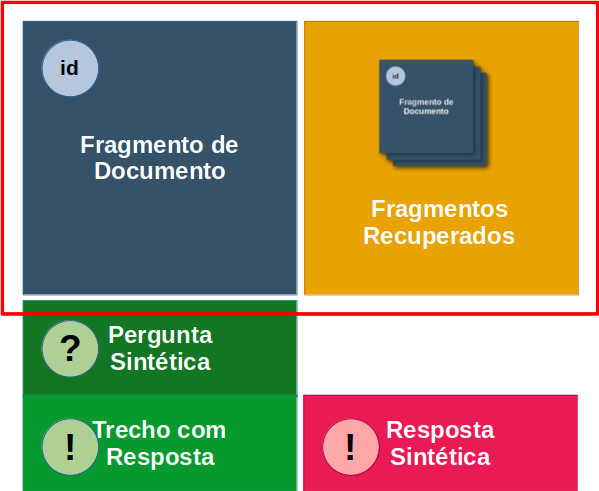
\includegraphics[width=0.5\linewidth]{Imagens/avaliacao-recuperacao.png}
    \caption{Mecanismo de avaliação da recuperação de documentos pelo banco vetorial}
    Fonte: autoria própria
    \label{fig:avaliacao-recuperacao}
\end{figure}

A Tabela \ref{tab:recuperacao-rank} apresenta a porcentagem de ocorrências de classificação do documento original em cada uma das posições do conjunto de documentos recuperados, para cada uma das três configurações testadas. A linha cuja posição é marcada como ``Ausente'' indica a quantidade de ocorrências em que o documento original não figurou entre os 10 documentos identificados pelos modelos como mais semanticamente semelhantes à consulta feita.

\begin{table}[H]
    \caption{Porcentagem de classificação do documento original em cada posição dos documentos recuperados}
    \centering
    \begin{tabular}{ c c c c }
        \hline
        \textbf{Posição} & \textbf{Sem Instrução} & \textbf{Português} & \textbf{Inglês} \\  
        \hline
        1ª & 1460 & 1009 & 939 \\
        2ª & 257 & 219 & 245 \\
        3ª & 129 & 124 & 125 \\
        4ª & 66 & 87 & 95 \\
        5ª & 53 & 65 & 66 \\
        6ª & 34 & 52 & 46 \\
        7ª & 32 & 41 & 46 \\
        8ª & 24 & 30 & 30 \\
        9ª & 15 & 22 & 39 \\
        10ª & 20 & 25 & 20 \\
        Ausente & 205 & 621 & 644 \\
        \hline
    \end{tabular}   
    
    Fonte: O autor (2024)
    \label{tab:recuperacao-rank}
\end{table}

A Tabela \ref{tab:recuperacao-acerto-erro}, por sua vez, demonstra a taxa de recuperação do documento original entre os 10 documentos recuperados do banco vetorial.

\begin{table}[H]
    \caption{Taxa de sucesso e falha na recuperação dos documentos originais por configuração}
    \centering
    \begin{tabular}{ c c c c c c }
        \hline
        \textbf{Pos} & \textbf{Ing Dif} & \textbf{Ing Igu} & \textbf{Por Dif} & \textbf{Por Igu} & \textbf{Base} \\  
        \hline
        Sucesso & 63,55\% & 60,65\% & 58,55\% & 54,56\% & 79,47\% \\
        Falha & 36,45\% & 39,35\% & 41,45\% & 45,44\% & 20,53\% \\
        \hline
    \end{tabular}
    
    Fonte: O autor (2024)
    \label{tab:recuperacao-acerto-erro}
\end{table}

As informações nas Tabelas \ref{tab:recuperacao-rank}  e \ref{tab:recuperacao-acerto-erro} sugerem que, apesar de um dos pontos fortes do \textit{instructor-xl} ser sua capacidade de geração de \textit{embeddings} adaptativos de alta qualidade sem a necessidade de \textit{fine-tuning} tradicional (Seção \ref{subsec:Assistente.1.2}), os resultados empíricos deste estudo apontaram para uma discrepância significativa entre o desempenho esperado e o observado, quando a funcionalidade sem ajuste fino foi comparada às versões ajustadas. Especificamente, a versão sem \textit{fine-tuning} demonstrou, em relação à versão com \textit{fine-tuning}, uma taxa de erro equivalente à metade da taxa de erro de todas as configurações de \textit{fine-tuning} nos casos analisados de recuperação de documentos com base na semelhança semântica, ao contrário do que se esperava, com base na premissa central do modelo.

Adicionalmente, é perceptível que a grande maioria das vezes em que o documento original estava entre os recuperados, figurou ele entre os 5 primeiros documentos. Isso nos permite avaliar que configurar o banco vetorial para retornar somente 5 registros por busca, dentro deste conjunto de dados, pode ser uma decisão segura, diminuindo a quantidade de dados a ser repassada para o \ac{LLM} gerar a resposta.

Um ponto adicional a se considerar sobre essa metodologia de teste automatizado de recuperação de documentos é o fato de as perguntas serem sintéticas, geradas por um \ac{LLM}. Uma averiguação pergunta a pergunta, explorando todos os mais de 4.000 casos, seria necessária para aferir a qualidade do seu conteúdo e sua efetiva correspondência com os artigos a partir dos quais elas foram geradas. Há, portanto, a possibilidade de, existindo perguntas mal formuladas, as taxas de falha na recuperação estarem superestimadas. Evidencia-se, assim, a importância de uma avaliação humana nesse sentido.

Por último, é importante considerar os casos em que respostas para uma pergunta específica estão em conteúdo distribuído em múltiplos artigos/fragmentos. Visto que as perguntas sintéticas foram criadas a partir de um fragmento específico e unicamente dele, não houve ocorrência desse tipo específico de questões nesta parte dos testes.

\subsection{Avaliando a Geração da Resposta}
\label{subsec:Resultados.2.2}

Considerando os resultados apontados na Seção \ref{subsec:Resultados.2.1}, que demonstram a melhor qualidade de recuperação de documentos utilizando a versão sem \textit{fine-tuning} do \textit{instructor-xl}, tal configuração foi a opção escolhida para se avaliar a geração de respostas do Assistente. Utilizamos como elementos de teste o conjunto de perguntas sintéticas geradas por meio do que se descreveu na Seção \ref{sec:Metodologia.4}, juntamente com o trecho do fragmento de documento apontado pelo GPT-4o como contendo o teor de resposta, quando do processo de geração das perguntas. Acrescentados a isso, foi o conjunto de documentos resultantes da consulta feita no Chroma DB, utilizando cada uma das perguntas em questão.

A aferição da qualidade da geração de respostas aumentadas por recuperação de documentos foi realizada por meio do uso da ferramenta BERTScore. Para isso, para cada uma das perguntas sintéticas utilizadas para os testes, o texto de sua resposta gerada pelo Assistente foi submetido à comparação, por meio do BERTScore, com um análogo a um ``texto de referência'' / \textit{gold standard}. Diz-se análogo pelo fato de que, diferentemente de texto gerado ou anotado por um avaliador humano, o referencial utilizado foi o trecho de fragmento utilizado para geração da pergunta que contém a informação referente ao teor esperado da resposta (ver Figura \ref{fig:avaliacao-resposta-gerada}).

\begin{figure}
    \centering
    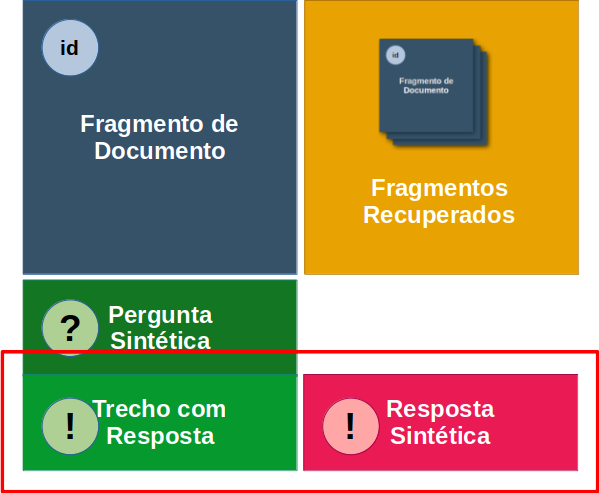
\includegraphics[width=0.5\linewidth]{Imagens/avaliacao-resposta-gerada.png}
    \caption{Mecanismo de avaliação de qualidade da resposta gerada}
    Fonte: autoria própria
    \label{fig:avaliacao-resposta-gerada}
\end{figure}

Para uma análise granular, o BERTScore foi aplicado sobre três porções do conjunto de perguntas/documentos recuperados/respostas. A primeira porção é correspondente às perguntas cujo conjunto de fragmentos de documentos recuperados do Chroma DB incluía o fragmento utilizado para gerar a pergunta (79\% do conjunto completo de perguntas), ao qual rotulamos, por conveniência como casos de \textbf{Sucesso} na recuperação. A segunda porção consiste das perguntas cuja resposta do Chroma DB não incluía do fragmento original (21\% do total de perguntas no conjunto), ao qual chamamos de casos de \textbf{Falha} na recuperação. A terceira aplicação foi sobre o conjunto completo, incluindo tanto os caso de sucesso ou falha, ao qual chamamos de \textbf{Dataset}.

A Tabela \ref{tab:bertscore-medias} mostra as médias de Precisão, \textit{Recall} e \textit{F1-Score} do BERTSccore para cada uma das aplicações. As Figuras \ref{fig:bertscore-sucesso}, \ref{fig:bertscore-falha} e \ref{fig:bertscore-dataset} mostram informações sobre a distribuição dos valores de cada pergunta para as porções de Sucesso, Falha e Dataset, respectivamente.

\begin{table}
    \caption{Médias da pontuação BERTScore por grupo de instâncias}
    \centering
    \begin{tabular}{ c c c c }
        \hline
        \textbf{Scores} & \textbf{Sucesso} & \textbf{Falha} & \textbf{Dataset} \\
        \hline
        Precisão & 79\% & 70\% & 77\% \\
        \textit{Recall} & 69\% & 63\% & 68\% \\
        F1-Score & 73\% & 66\% & 72\% \\
        \hline
    \end{tabular}
    
    Fonte: O autor (2024)
    \label{tab:bertscore-medias}
\end{table}

Naturalmente, para as três medidas (precisão, \textit{recall} e \textit{f1-score}, as respostas geradas a partir dos casos de sucesso na recuperação do documento base original obtiveram valores mais altos que os casos de falha. Sua taxa de precisão com valor de 79\% aponta para um bom alinhamento das informações na resposta gerada com o trecho de documento que contém a informação da resposta desejada. Ao mesmo tempo, o \textit{recall} de 69\% indica um nível satisfatório de cobertura do teor da resposta alvo.

A despeito dos valores mais baixos nos casos de falhas, a média geral da qualidade das respostas às perguntas do conjunto como um todo foram também satisfatórias. Não obstante, uma avaliação humana das respostas e seleção de documentos retornados do banco vetorial pode dar mais informações dos pontos de falha do Assistente.

Adicionalmente, é relevante apontar que as pontuações do BERTScore de precisão e \textit{recall}, diferentemente de outras aplicações, somente tendem a ficar com valores muito próximos de 1 quando da correspondência exata das palavras da resposta gerada com as palavras da resposta desejada. Mesmo em casos de respostas corretas, geradas por atores humanos, é incrementalmente mais improvável a redação de uma resposta a uma pergunta com teor exatamente igual a um texto de referência, salvo em casos de citação direta. 

\begin{figure}
    \centering
    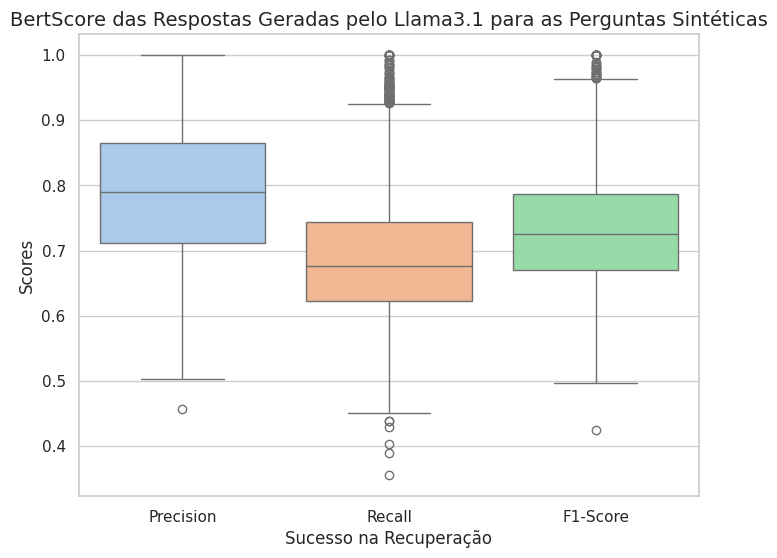
\includegraphics[width=0.5\linewidth]{Imagens/bertscore-sucesso.png}
    \caption{Pontuação BERTScore do conjunto de casos de sucesso na recuperação do documento original}
    Fonte: autoria própria
    \label{fig:bertscore-sucesso}
\end{figure}

\begin{figure}
    \centering
    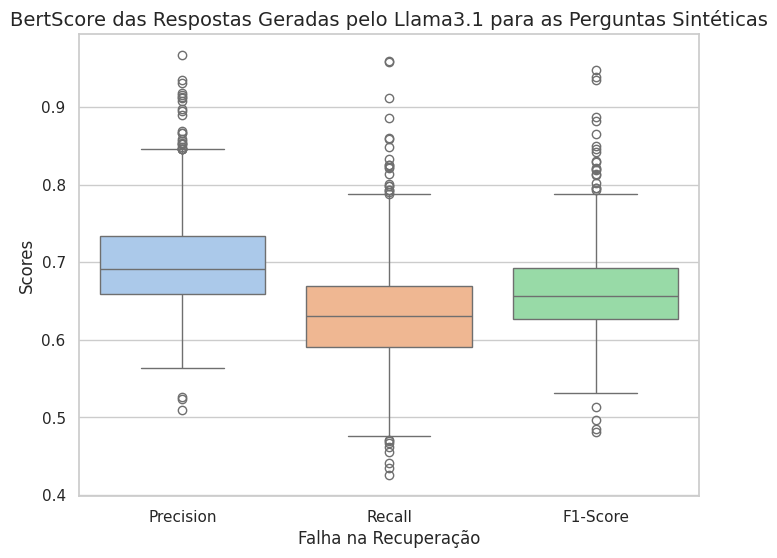
\includegraphics[width=0.5\linewidth]{Imagens/bertscore-falha.png}
    \caption{Pontuação BERTScore do conjunto de casos de falha na recuperação do documento original}
    Fonte: autoria própria
    \label{fig:bertscore-falha}
\end{figure}

\begin{figure}
    \centering
    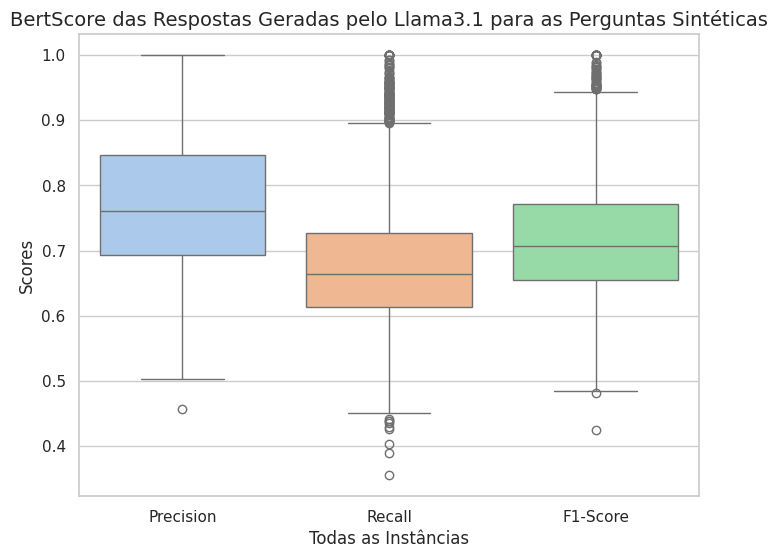
\includegraphics[width=0.5\linewidth]{Imagens/bertscore-dataset.png}
    \caption{Pontuação BERTScore do conjunto de dados inteiro}
    Fonte: autoria própria
    \label{fig:bertscore-dataset}
\end{figure}

\subsection{Tempo de Performance}
\label{subsec:Resultados.2.3}

Os experimentos de testes descritos neste estudo foram implementados por meio de \textit{scripts} desenvolvidos na linguagem de programação Python e armazenados em um repositório público no GitHub, tanto para fins de transparência, quanto para fins de agilizar e simplificar o processo de execução, independente do local e da máquina utilizada. Devido à indisponibilidade de hardware local adequado para a execução dos testes, especialmente considerando a alta demanda computacional associada à utilização de modelos de \ac{LLM}s em execução paralela com uma instância do Ollama com o Llama 3.1, optou-se por clonar o repositório em instâncias do Google Colab para a condução dos experimentos. Essa abordagem garantiu acesso a recursos computacionais avançados, mitigando as limitações do ambiente local.

O ambiente de execução no Google Colab foi configurado com uma GPU NVIDIA T4, que dispõe de 16 GB de memória dedicada, sendo a configuração padrão de utilização gratuita da plataforma. Essa arquitetura foi fundamental para permitir a execução eficiente de modelos pesados, assegurando um desempenho adequado tanto para o processo de recuperação de documentos do banco vetorial, quanto para a execução do modelo Llama para gerar as respostas. A integração entre os recursos oferecidos pelo Google Colab e as capacidades do Ollama foi configurada de forma a maximizar a compatibilidade e o desempenho dos experimentos.

Por meio dessa infraestrutura, foi possível realizar os testes necessários sem comprometer a validade dos resultados, assegurando que a execução dos experimentos fosse realizada de maneira confiável e reprodutível. Adicionalmente, a utilização do repositório GitHub como plataforma para versionamento e controle do código contribuiu para a transparência e rastreabilidade das implementações, elementos essenciais em um contexto de pesquisa científica.

Nesse contexto, foram coletadas estatísticas do tempo de execução das etapas mais custosas de todo o processo, a saber, a recuperação de documentos do banco vetorial Chroma DB e, especialmente, a geração de respostas por meio do Llama. Conforme Figura \ref{fig:tempo-chroma}, a média de tempo de recuperação de documentos ficou em 0,05 segundos. O Llama, por sua vez, teve uma média de tempo de geração de perguntas de pouco mais de 4,5 segundos.

Curiosamente, na Figura \ref{fig:distribuicao-chroma}, é possível notar que a distribuição do tempo de resposta do Chroma DB aponta para duas faixas distintas de tempo de resposta, com médias em torno de 0,045 segundos e 0,064 segundos. Investigação mais aprofundada é necessária para entender esse fenômeno.

\begin{figure}
    \centering
    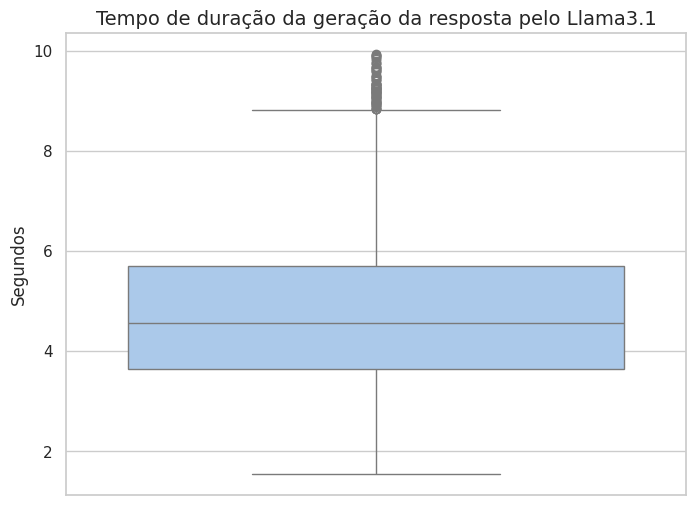
\includegraphics[width=0.5\linewidth]{Imagens/llama.png}
    \caption{Tempo de Geração da Resposta pelo Llama}
    Fonte: autoria própria
    \label{fig:tempo-llama}
\end{figure}

\begin{figure}
    \centering
    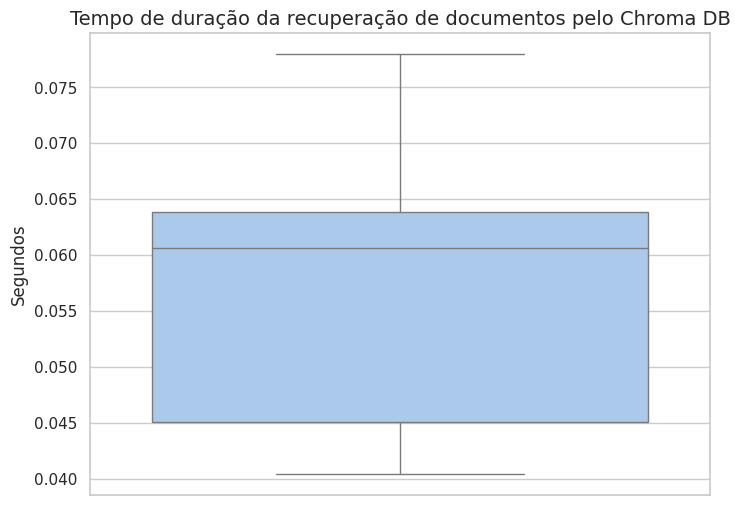
\includegraphics[width=0.5\linewidth]{Imagens/chroma.png}
    \caption{Tempo de Recuperação de Documentos pelo Chroma DB}
    Fonte: autoria própria
    \label{fig:tempo-chroma}
\end{figure}

\begin{figure}
    \centering
    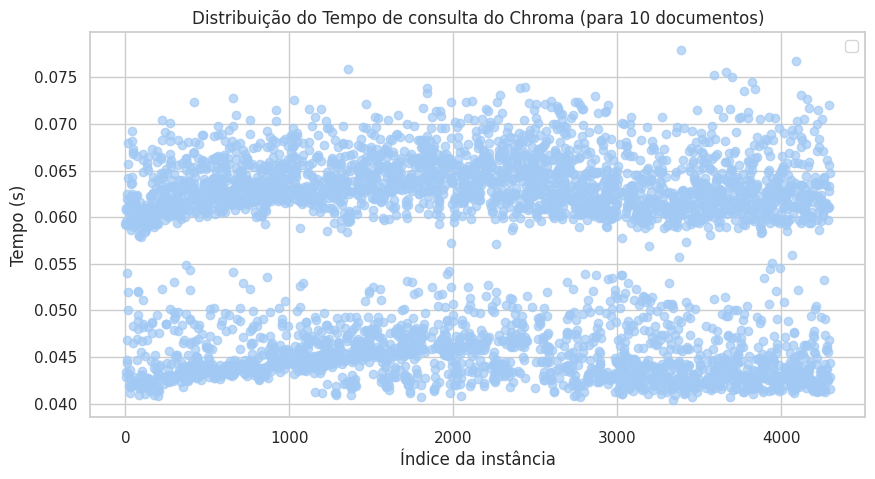
\includegraphics[width=0.75\linewidth]{Imagens/distribuicao_chroma.png}
    \caption{Distribuição do Tempo de Recuperação do Chroma DB}
    Fonte: autoria própria
    \label{fig:distribuicao-chroma}
\end{figure}

\section{Avaliações Humanas da Abordagem RAG}

As avaliações humanas ainda estão sendo implementadas.